% Options for packages loaded elsewhere
\PassOptionsToPackage{unicode}{hyperref}
\PassOptionsToPackage{hyphens}{url}
%
\documentclass[
]{article}
\usepackage{lmodern}
\usepackage{amssymb,amsmath}
\usepackage{ifxetex,ifluatex}
\ifnum 0\ifxetex 1\fi\ifluatex 1\fi=0 % if pdftex
  \usepackage[T1]{fontenc}
  \usepackage[utf8]{inputenc}
  \usepackage{textcomp} % provide euro and other symbols
\else % if luatex or xetex
  \usepackage{unicode-math}
  \defaultfontfeatures{Scale=MatchLowercase}
  \defaultfontfeatures[\rmfamily]{Ligatures=TeX,Scale=1}
\fi
% Use upquote if available, for straight quotes in verbatim environments
\IfFileExists{upquote.sty}{\usepackage{upquote}}{}
\IfFileExists{microtype.sty}{% use microtype if available
  \usepackage[]{microtype}
  \UseMicrotypeSet[protrusion]{basicmath} % disable protrusion for tt fonts
}{}
\makeatletter
\@ifundefined{KOMAClassName}{% if non-KOMA class
  \IfFileExists{parskip.sty}{%
    \usepackage{parskip}
  }{% else
    \setlength{\parindent}{0pt}
    \setlength{\parskip}{6pt plus 2pt minus 1pt}}
}{% if KOMA class
  \KOMAoptions{parskip=half}}
\makeatother
\usepackage{xcolor}
\IfFileExists{xurl.sty}{\usepackage{xurl}}{} % add URL line breaks if available
\IfFileExists{bookmark.sty}{\usepackage{bookmark}}{\usepackage{hyperref}}
\hypersetup{
  pdftitle={York Biology Journal Club},
  hidelinks,
  pdfcreator={LaTeX via pandoc}}
\urlstyle{same} % disable monospaced font for URLs
\usepackage[margin=1in]{geometry}
\usepackage{graphicx,grffile}
\makeatletter
\def\maxwidth{\ifdim\Gin@nat@width>\linewidth\linewidth\else\Gin@nat@width\fi}
\def\maxheight{\ifdim\Gin@nat@height>\textheight\textheight\else\Gin@nat@height\fi}
\makeatother
% Scale images if necessary, so that they will not overflow the page
% margins by default, and it is still possible to overwrite the defaults
% using explicit options in \includegraphics[width, height, ...]{}
\setkeys{Gin}{width=\maxwidth,height=\maxheight,keepaspectratio}
% Set default figure placement to htbp
\makeatletter
\def\fps@figure{htbp}
\makeatother
\setlength{\emergencystretch}{3em} % prevent overfull lines
\providecommand{\tightlist}{%
  \setlength{\itemsep}{0pt}\setlength{\parskip}{0pt}}
\setcounter{secnumdepth}{-\maxdimen} % remove section numbering

\title{York Biology Journal Club}
\author{}
\date{\vspace{-2.5em}}

\begin{document}
\maketitle

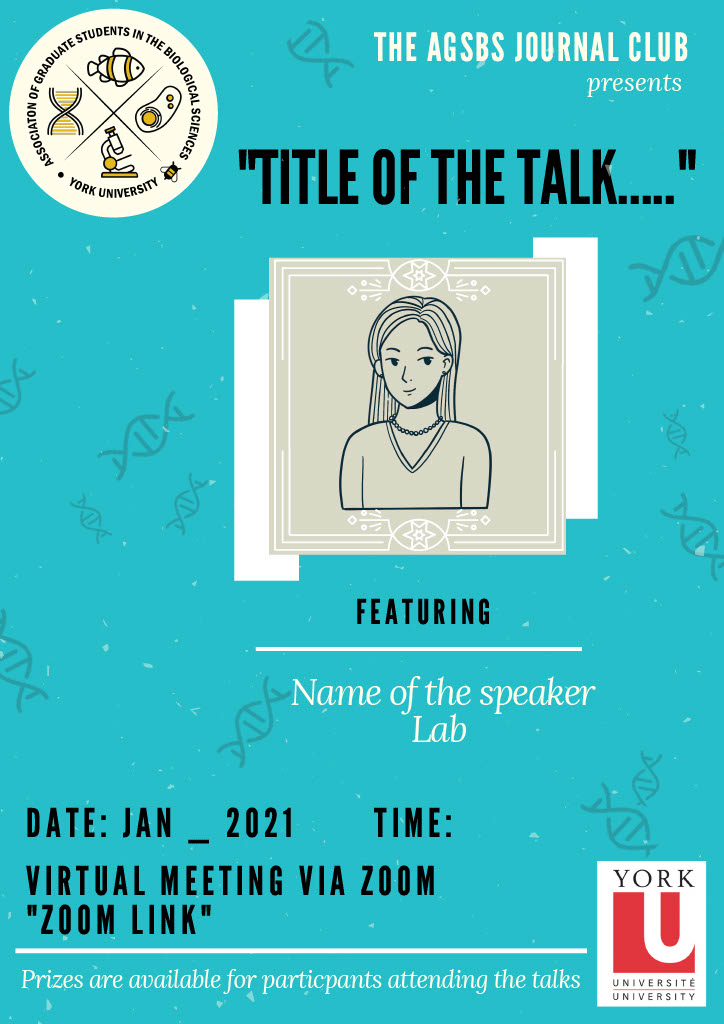
\includegraphics{template1.jpg}

\hypertarget{hello}{%
\subsection{Hello!}\label{hello}}

The journal club committee invites you to get involved with the AGSBS
Departmental Journal Club in 2021.

There will be eight monthly, one hour sessions between January and
August and two student presenters per session. The sessions will be held
online using Zoom, on the last Friday of each month at 12 pm. Each
presenter has up to 30 minutes -- present your own work with a question
and answer session, or present a paper of your choice and lead a
discussion -- or any combination of the two! Each presenter will receive
a gift card of their choice worth \$20. In addition, here will be a
prize raffle at the end of each session for three lucky attendees. Come
out and support your fellow graduate students!

We encourage all speakers to make their talks accessible and interesting
to those in all areas of biology. We welcome talks on a very wide range
of topics. For example, tell us about the project you are working on, or
that new ground-breaking paper within your discipline. Lead a discussion
on a controversial paper, a paper addressing science as a career choice
or anything else! This is a supportive space for all graduate students!

\hypertarget{sign-up-to-be-a-discussion-leader}{%
\subsection{Sign up to be a Discussion
Leader}\label{sign-up-to-be-a-discussion-leader}}

Sign up as a presenter using this google form and send us an email if
you have any questions. You do not need to have decided on a topic to
sign up.
\href{https://docs.google.com/forms/d/e/1FAIpQLSdAdlvA4kEKg68sLV6CCKkBobYLIipfGbs_FrUJab_jkkqqiQ/viewform?usp=sf_link}{Sign
up here!}

Zoom links will be sent out via the Biograds listserve prior to the
event.

\hypertarget{committee-members}{%
\subsubsection{Committee members}\label{committee-members}}

\begin{itemize}
\tightlist
\item
  Jenna Braun
\item
  Malory Owen
\item
  Cindy Tran
\item
  Marjan Moallem
\item
  David Miller
\end{itemize}

\end{document}
